\section{Metabolizer}

Consider alcohol dehydrogenase, whereby an -OH group, connected to
a chemical substructure R of arbitrary complexity, loses its Hydrogen
and becomes an =O group. The first line of the database shows how
this general reaction is currently stored in the pathway tools database:

\vspace{.1in}

\begin{center}\includegraphics[
  scale=0.4]{dehydrog.eps}\end{center}

\vspace{.1in}

The second line is the same reaction at a structural level. An instance
of this general reaction -- ethanol -> acetaldehyde -- is shown on
the third and fourth lines.

Clearly, to be able to recognize the pattern/instance relationship
between these two reactions, knowledge of the chemicals' structural
representations is necessary; there is no deducible relationship between
the atomic symbols 'alcohol and 'ethanol. In our current approach
we therefore have no means of representing this general-level chemical
knowledge. Our database is often bloated with repetitive instances
of a small set of patterns. Worse, it is incomplete: in the case of
alcohol dehydrogenase, for example, there is no way that the database
has populated a corresponding aldehyde for every single chemical entry
that has an -OH group.

An extension to our project, one that we made a minor dent on, would
be to move our database from a reaction-of-names to a reaction-of-structures
representation. Such a move would naturally allow such generic chemical
knowledge to be encoded. The idea is to create a dynamic database
that expands as reactions are explored throughout a search, through
the application of appropriate generic reactions to the current chemicals
at hand. The generic reactions, applied to specific reactants, produce
specific products that can be added to the database.

The set-up we propose is to use graph pattern matching to figure out
when a generic reaction applies, and to use graph rewriting to derive
the products that result. Two procedures, MATCH and REWRITE, would
provide this behavior.

We started attempting to write MATCH using combinator-style syntactic
pattern matching. We chose to represent chemical structure graphs
using adjacency lists. CO2, for example, looks like:

((C (2 2) (3 2)) 
 (O (1 2)) 
 (O (1 2))) 

 Where the C has index 1, and the Os have index 2 and 3 respectively. The C
 entry indicates that it is bonded to atom 2, that it is a double-bond, and
 likewise for atom 3. The remaining entries redundantly reflect the same
 connectivity.  We thought about using canonicalization -- alphabetical
 atom ordering, with increasing-index order for the bond lists of each
 entry. Unfortunately, a single chemical can still have several different
 adjacency lists under this canonicalization (for example C=0=C=0=C), so
 syntactic pattern matching would require combinatorially many patterns to
 work correctly.

It turns out several hours in the lab saved us 30 minutes in the library.
Looking through Pathway Tools, we found an ancient subgraph matcher
that could do precisely what we wanted. It works by aligning two atoms
in the two input patterns, seeing if their bonds are consistent, and
recursing on the atoms at the end of each bond, backtracking when
necessary. We wrote a quick wrapper to provide the interface we desired
and to hide hairiness of the underlying code.

The next step, one we may pursue in the future, is the REWRITE procedure.
The design we had in mind is as follows:

\vspace{.1in}

\begin{center}\includegraphics[
  scale=0.4]{rewrite.eps}\end{center}

\vspace{.1in}

In addition to the specific reactants, we have two pieces of information
to work with as input to REWRITE: our generic reaction, represented
as an atom mapping from generic reactants to generic products, and
our MATCH to the specific reactants, also represented as a mapping.
The REWRITE procedure would combine these two mappings to figure out
how to rewrite the specific reactants into specific products. We may
be better served thinking about how to create a better language for
describing the mappings, rather than using atom number mappings. Currently,
the task of coding REWRITE seems both daunting and not particularly
stimulating. 

